%\vfill\eject
%\newpage
\chapter[The Focal Plane Polarimeter]{The Focal Plane Polarimeter
\footnote{
  $CVS~revision~ $Id: fpp.tex,v 1.7 2003/12/17 03:59:48 gen Exp $ $
}
\footnote{Authors: S.Nanda \email{nanda@jlab.org}}
}

\section{Overview}

The focal plane polarimeter measures the polarization of protons in the
hadron spectrometer detector stack.
When the protons pass through a carbon analyzer, the nuclear spin-orbit
force leads to an azimuthal asymmetry in scattering from carbon nuclei,
if the protons are polarized. 
The particle trajectories, in particular the
scattering angles in the carbon, are determined by pairs of front and rear
straw chambers, a type of drift chamber.

As shown in Figure~\ref{fig:hadron_det}, 
the front straw chambers are separated by about 114 cm, and are located
before and after the gas \Cherenkov{} detector.
The second chamber is followed by scintillator 2, which is in turn
followed by the polarimeter carbon analyzer.
The rear chambers, chambers 3 and 4, are separated by 38 cm and are
immediately behind the carbon analyzer.

\begin{figure}[bth]
\begin{center}
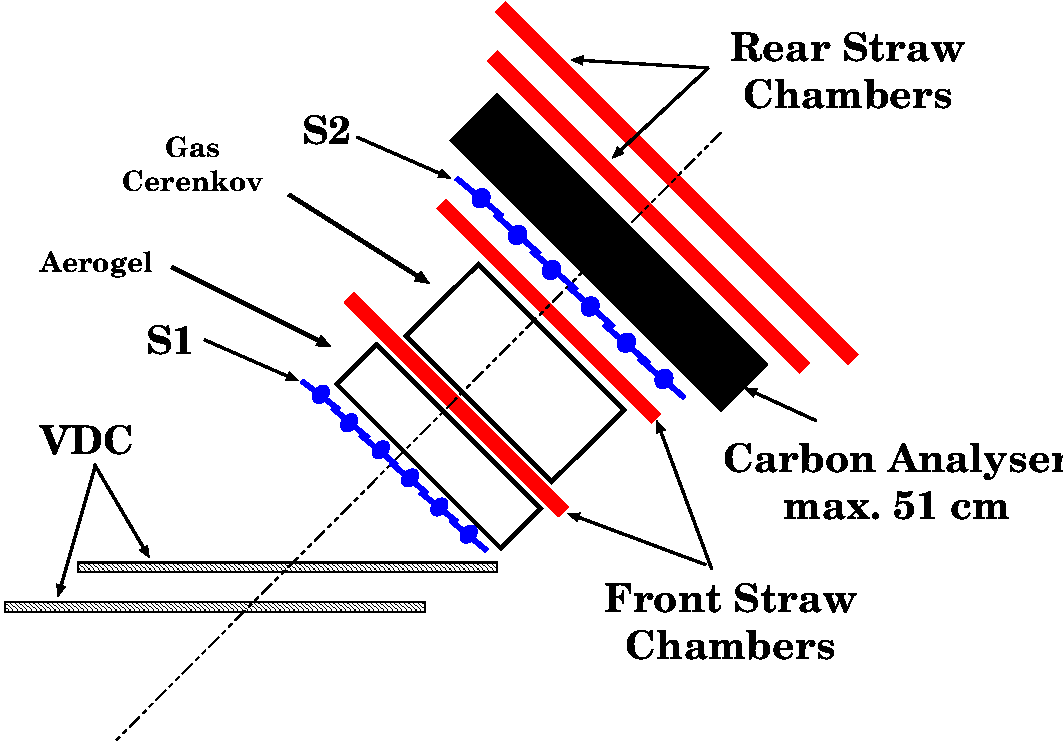
\includegraphics[angle=0,width=15cm,clip]{hadrondeteng}
{\linespread{1.}
\caption[Detectors: Hadron Arm detector]{Schematic of the hadron detector stack.}
\label{fig:hadron_det}}
\end{center}
\end{figure}

The carbon analyzer consists of 5 carbon blocks.
Each block is split in the middle so that it may be moved into or out
of the proton paths, so that the total thickness of scattering carbon may be
adjusted.
The block thicknesses, from front to rear, are 9" (22.9cm), 6" (15.2cm), 
3" (7.6cm) , 1.5" (3.8cm) , and 0.75" (1.9cm).
The block positions are controlled through EPICS~\cite{EPICSwww}; the controls
may be reached through the Hall A / hadron spectrometer / detectors menus%
\infolevtwo{ (see Fig.~\ref{fig:medm-hlamain-tools})}.
Particles passing through the carbon analyzer can be absorbed in it.

The straw chamber planes are designated as X, U, and V planes.
The central ray defines the z axis.
X wires measure position along the dispersive direction.
The UV coordinate system is created by a 45 degree rotation in the
transverse plane of the XY coordinate system, with +U between the
+X and +Y axes, and +V between the +Y and -X axes.

\infolevthree{
The straw chamber operation is described in the following paragraphs.

When a charged particle passes through the chamber in typical Jefferson Lab
operating conditions, there will be about 30 primary ionizations of gas
molecules.
Positive high voltage of about 1.8 - 1.9 kV is applied to the wire in the
center of each straw.
Electrons from the ionizations drift towards the wire.
When the electrons get within about 100 $\mu$ of the wire, the gain in energy
between collisions with gas molecules is sufficient that gas molecules
are further ionized in collisions.
This leads to an {\it avalanche}, and a gain of about 
10$^5$ per primary ionization under the conditions in which the FPP is run.

The movement of the positive and negative ions leads to a voltage drop
on the wire, or equivalently to a negative analog signal.
The analog signal is about 20 ns long, with a (negative)
peak current of about 40 $\mu$A, and propagates towards each end of the straw.
} %infolev
\infolevone{
At one end of each straw is a board that supplies high voltage
(see Figure \ref{fig:termboard});
impedance matching on this board, with a 1500 pF capacitor and a 370 $\Omega$
resistor, reduces reflection of the signal.

\begin{figure}[tbh]
\begin{center}
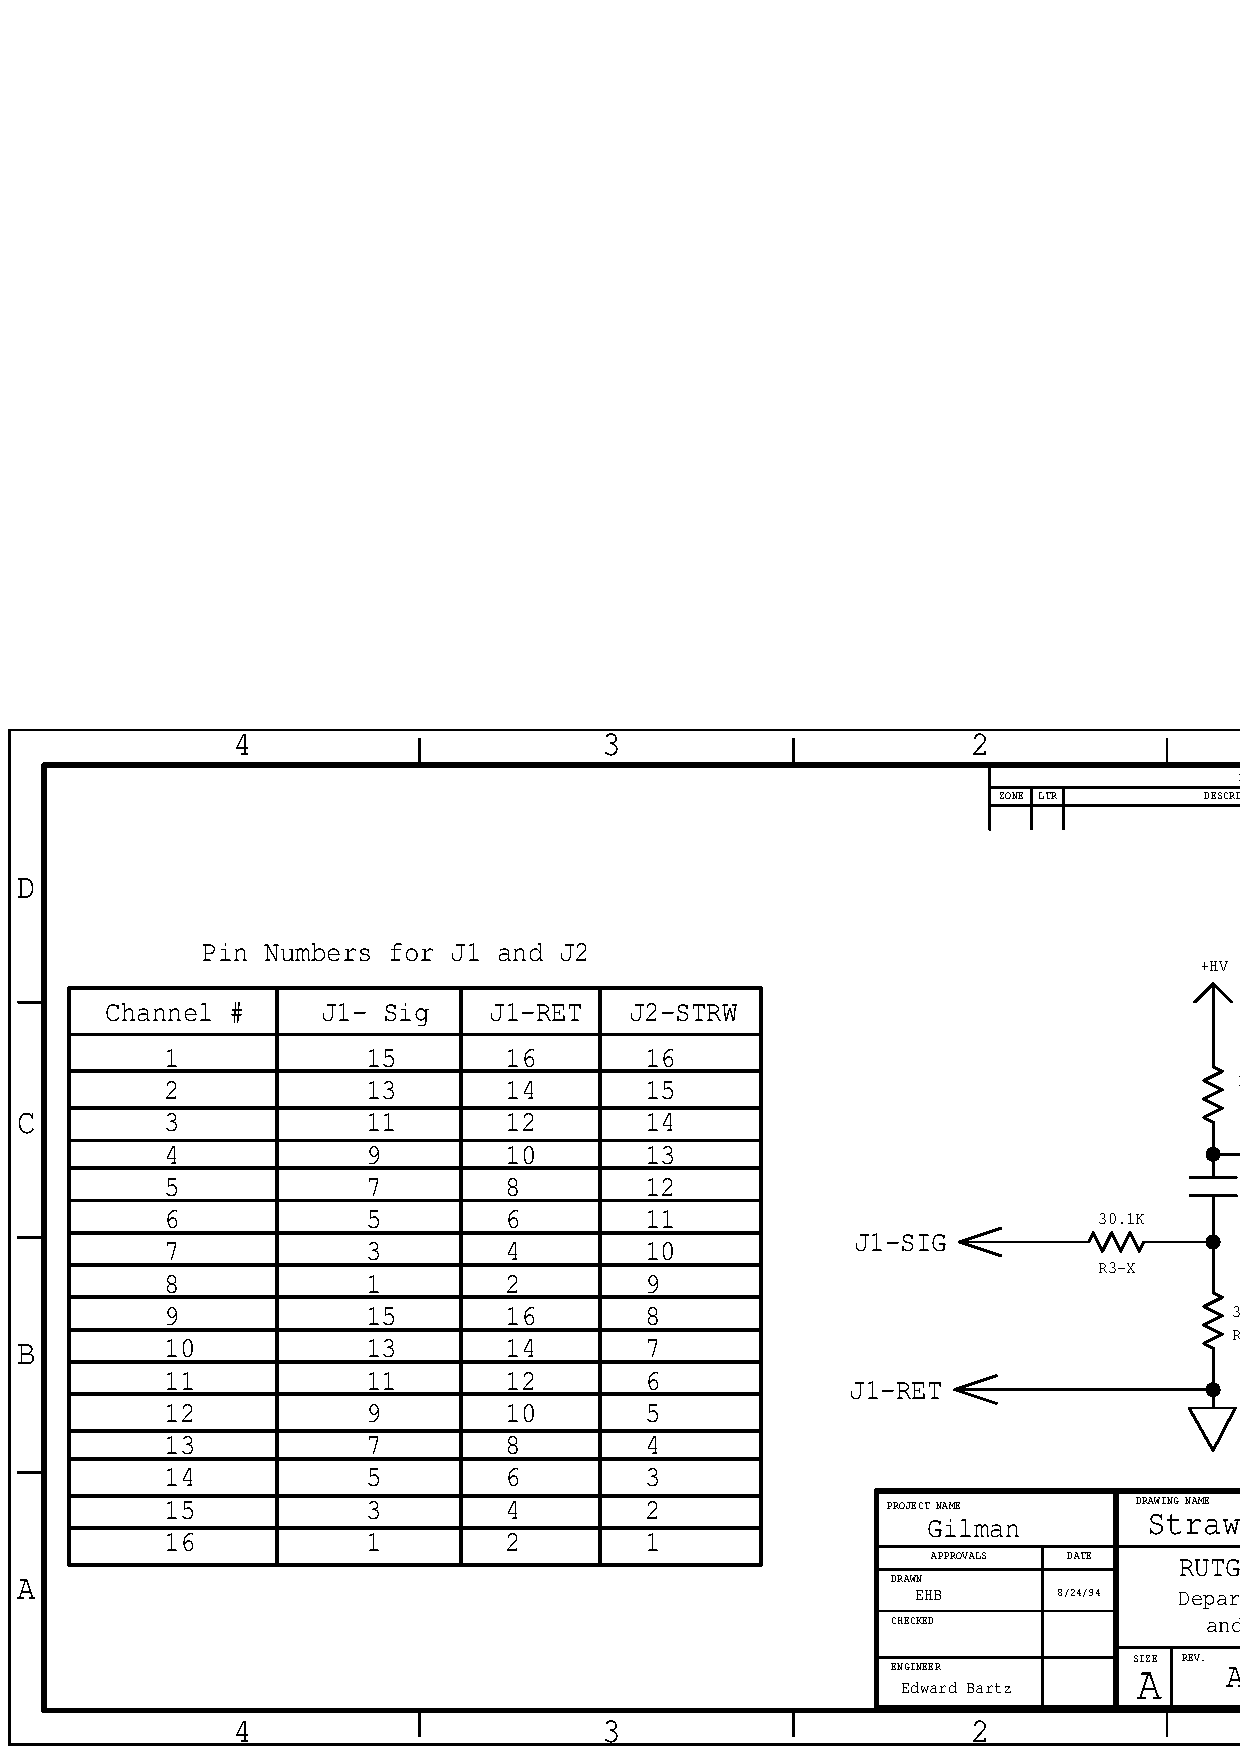
\includegraphics[angle=0,width=\textwidth]{fpp_term_board}
{\linespread{1.}
\caption[Detectors: FPP HV Termination Board]{Circuit diagram for the high voltage / termination board.}
\label{fig:termboard}}
\end{center}
\end{figure}

The other end of each straw is connected to a readout board, that amplifies,
discriminates, and multiplexes the input signals --
(see Figures \ref{fig:readoutboard1} and \ref{fig:readoutboard2} ).
At the readout end, the signal is ``coupled to ground'' through a 1500
pF capacitor followed by 310 $+$ 50 $\Omega$ resistors.
In parallel with the 50 $\Omega$ resistor are diodes to limit the
signal size, preventing damage to the readout board circuitry.
An amplifier samples the signal over the 50 $\Omega$ resistor.
The amp gain is about -10 mV/$\mu$A, resulting in a +400 mV signal
to a comparator.
A threshold voltage input to the readout board is put over a voltage divider
consisting of 1500 $+$ 10 $\Omega$ resistors.
For the typical 4 V threshold applied to the board, the comparator
puts out a logical pulse when the 400 mV (peak) signal rises above the
4 V / 151 = 26 mV threshold.
One-shots are then used to fix the width of the logical pulse for each channel
-- the one-shot width is fine tuned by the use of high precision resistors in
an RC circuit; these resistors are mounted in sockets so as to be easily
replaced if the need arises.
An OR circuit then combines eight individual straw outputs into a single
electronics channel.

\begin{figure}
\begin{center}
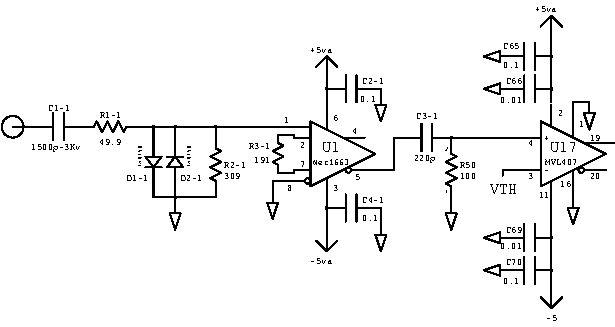
\includegraphics[angle=0,width=\textwidth]{fpp_readout_board_t_1}
{\linespread{1.}
\caption[Detectors: FPP Readout Board]{Circuit diagram for the
amplifier / discriminator section of the readout board.}
\label{fig:readoutboard1}}
\end{center}
\end{figure}

\begin{figure}
\begin{center}
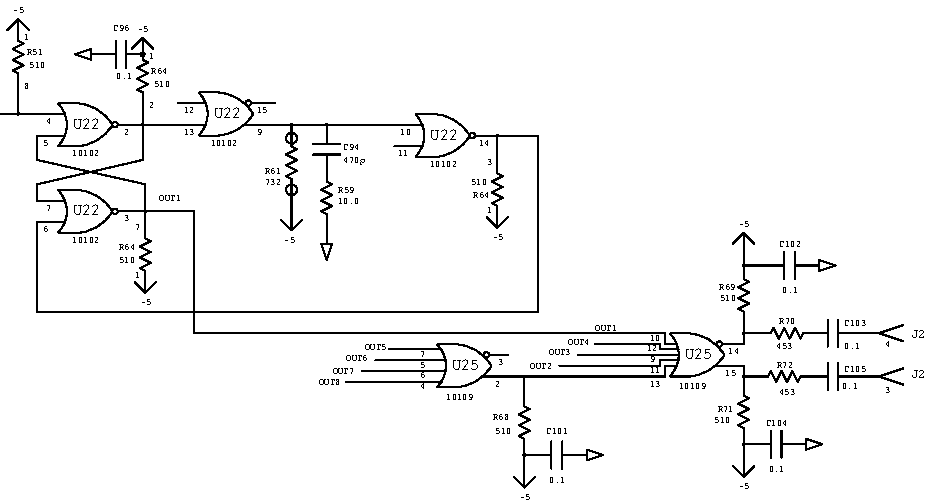
\includegraphics[angle=0,width=\textwidth]{fpp_readout_board_t_2}
{\linespread{1.}
\caption[Detectors: FPP Readout Board]{Circuit diagram for the
logical / multiplexing section of the readout board.}
\label{fig:readoutboard2}}
\end{center}
\end{figure}
Internally, within the Faraday cages, the high voltage is distributed to
stacks of high voltage / test pulser boards, through which it is connected to
each straw via a 1 M$\Omega$ 1/4 watt resistor.

The readout cards require a high-current low-voltage
power supply and a low-current low-voltage power
supply for a threshold level.
The readout electronics are mounted on the chamber, shielded
within Faraday cages.
The high-current power supplies were built by the Rutgers University
Department of Physics \& Astronomy Electronics Shop.
These supplies are set to provide sufficient current at $\pm$5 V for the
boards to which they are hooked up.
No adjustments, except for turning the supplies on / off, should be needed
in normal operation.
There are voltage setting, current limiting, and overvoltage protection
potentiometers within the boxes; adjustment information is given in the
FPP logbooks.
The low current supplies are {\em Hewlett-Packard} 6111A supplies.
The 6111As can provide up to 1 A for voltage from 0 to 20 V.
The supplies are currently hooked up through the rear panel to a DAC in
the data acquisition panel; front panel controls on the supplies are
disabled, except for the on/off switch.
The voltage is controlled through an EPICS FPP threshold window, that
is accessed through the Hall A / hadron spectrometer / detectors menus.
The high-current supplies are not computer controlled.
All supplies are mounted in the detector stack.

The multiplexed logical signals from the chambers have amplitudes
smaller than ECL levels, to prevent noise at the chamber.
These signals are fed to level shifter boards 
(see Figure \ref{fig:receiverboard}),
located in the FPP rack on
the lower electronics level of the detector stack, on the beam right side.
A high-current $\pm$5 V power supply for the level shifter boards is
located at the bottom of the same rack.
The boards convert the signals to ECL standard levels.
The level shifter outputs
are connected to the starts of {\em LeCroy} Model 1877 FASTBUS TDCs, located
in the lower electronics level on the beam left side.
The TDCs measure both leading and trailing edge times to allow demultiplexing.
The TDCs are subsequently stopped by the overall event trigger, and
are read out by the {\it CODA} acquisition software.
The data are histogrammed online by the {\it DHIST} software.
In-depth offline data analysis requires the {\it ESPACE} software.

\begin{figure}
\begin{center}
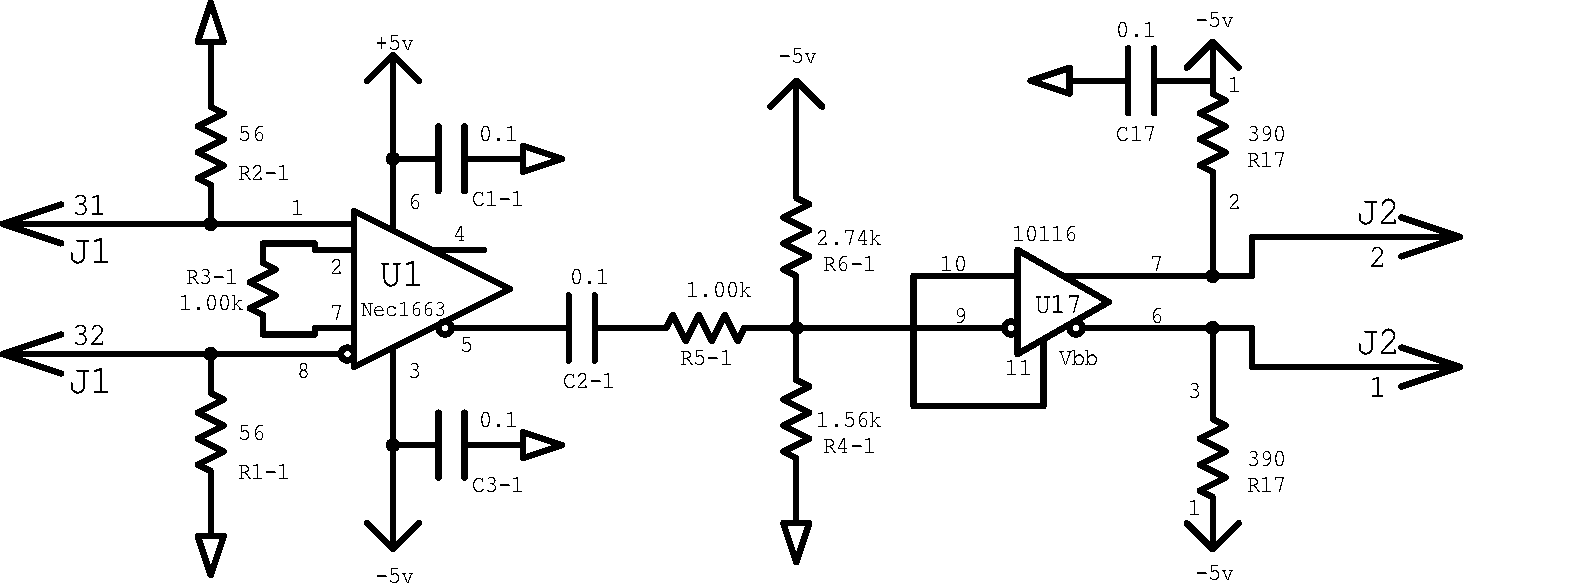
\includegraphics[angle=0,width=\textwidth,clip]{fpp_receiver_board_t}
{\linespread{1.}
\caption[Detectors: FPP Level Shifter Receiver Board]{Circuit diagram for the level shifter / receiver board.}
\label{fig:receiverboard}}
\end{center}
\end{figure}


The chamber gas is presently a combination of argon and ethane,
about 63\% and 37\% by weight. The Hall A gas shed is outside
next to the entrance of the Hall A truck ramp.
Gas is routed from the Hall A gas shed mixing system to the gas panel
located on the lower electronics level of the space frame, and subsequently
to the FPP chambers.
The gas system is shared with the VDCs.
A detailed description of the system has been written by
Howard Fenker\htmladdnormallinkfoot{}{\url{
http://www.jlab.org/Hall-A/document/HAWGS/HAWGS_OpMan.html
}}.

In addition, the chambers are outfitted with a test pulser capability.
A pulse is introduced into an 8 channel (16 wire) twisted pair cable
on each chamber, which connects to the high voltage boards,
at the opposite ends of each straw from the readout boards.
The pulse is resistively coupled through a 20 k$\Omega$ resistor
to the ground leg of a 1500 pF capacitor, and thence into the
straws.
After propagating through the straw, the pulse enters the readout board.
A pulse of about 1 V amplitude in the twisted pair cable is sufficient to
provide a few mV signal into the readout boards, resulting in a logical
output signal.
The system may be used to test the functionality of each readout channel
and / or the continuity of the high voltage wire in each straw.
The system currently is only implemented for manual operation, except
that data may be read out through CODA.
This procedure requires some familiarity with trigger logic and setup,
should only be done by experts, and is not documented here.
} %infoolev

\infolevtwo{
\section{Operating Procedure}
\paragraph {Gas Flow Operating Procedures}

The chamber gas is mixed 63$\%$-37$\%$ (by weight) Ar ethane. The gas is mixed
in the Hall A gas shed which is located next to the entrance to the 
Hall~A truck ramp. One needs key \#8, which is located in a key box 
in the Hall~A counting house, to get inside the shed 
where the gas mixing is done. 
The argon and ethane
bottles which feed the gas mixing system are located outside the shed
and can be exchanged when they are empty. The mixed gas is sent down into
Hall~A and to each of the detector huts. There are two each of argon and
ethane bottles connected to the gas system and a   Matheson 8590 controller
switches between the two bottles when the gas pressure in the bottle
drops below  a certain level. At this point the one bottle can be replaced 
while the other is being used. The procedure for changing gas bottles
is outlined below: 
\begin{enumerate}
\item Warning: High pressure gas bottles contain significant 
stored energy and are potentially hazardous. Handling of gas bottles 
should be done only by qualified, trained personnel.

\item For smoothest operation, used gas bottles should be 
replaced before their internal pressure drops below the desired 
regulator output pressure.

\item Two possible cases exist in which a gas bottle needs 
to be replaced: only one empty gas bottle on a system or 
both bottles empty on a gas system.

\item For case 1 the sequence of steps is as follows:

\begin{enumerate}
     \item Check in the Hall A Gas Shed. If all bottles have 
sufficient pressure each of the Matheson 8590 controllers 
will have one green "RUN" LED lit and one yellow "READY" LED lit. 
A red "EMPTY" LED lit indicates a bottle with low pressure, the 
corresponding bottle needs to be replaced. If a red "EMPTY" LED is lit 
the central "ALARM" LED should also show red. Nothing further needs 
to be done here; go outside to the Gas Bottle Pad. 

    \item Visually verify that the corresponding pressure gauge on 
the flex line is showing a low pressure. A low pressure is not 
necessarily zero. Close the bottle valve for the empty bottle.

    \item Disconnect the empty bottle from the high-pressure flex-line. 
The in-line check-valves will prevent gas escaping from the manifold. 
Replace the bottle's cap, and move the empty bottle to the EMPTIES 
storage rack. Note that ethane bottle fittings, type CGA-350, have 
left-handed threads.

    \item Place a full bottle of gas in the on-line rack, remove the 
bottle cap, and connect the bottle to the flex-line.

    \item Open the new bottle's valve, check for leaks at the bottle 
fitting. The corresponding pressure gauge should now read full bottle pressure.

    \item The ALARM state of the Matheson 8590 controller should have 
automatically reset. Check inside the Hall A Gas Shed. Each controller 
should show a green "RUN" and yellow "READY" LED lit. If not, 
re-check the installation of the gas bottle.
\end{enumerate}

\item For case 2 the sequence of steps is as follows:
\begin{enumerate}
    \item  Check in the Hall A Gas Shed. If all bottles have sufficient 
pressure each of the Matheson 8590 controllers will 
have one green "RUN" LED lit and one yellow "READY" LED lit. 
If a Matheson 8590 controller shows two red "EMPTY" LEDs lit and 
the central red "ALARM" LED lit, both bottles of the corresponding 
manifold need to be replaced. Nothing further 
needs to be done here, go outside to the Gas Bottle Pad. 

    \item Follow steps 2. through 5., as detailed immediately above, for 
both bottles.

    \item The ALARM state of the Matheson 8590 controller should have 
automatically reset. Check inside the Hall A Gas Shed. Each 
controller should show two yellow "READY" LEDs lit. If not, re-check 
the installation of the gas bottle. Press either of the two buttons 
labeled "LEFT BANK" and "RIGHT BANK". The lit LED above the button 
you pressed will change from yellow "READY" to green "RUN". You will 
most likely need to reset the Low Supply Pressure shutdown at this point.
\end{enumerate}
\end{enumerate}


The four FPP straw chambers are connected in parallel to the gas system.
(see Figure \ref{fig:gaspanel}).

\begin{figure}
\begin{center}
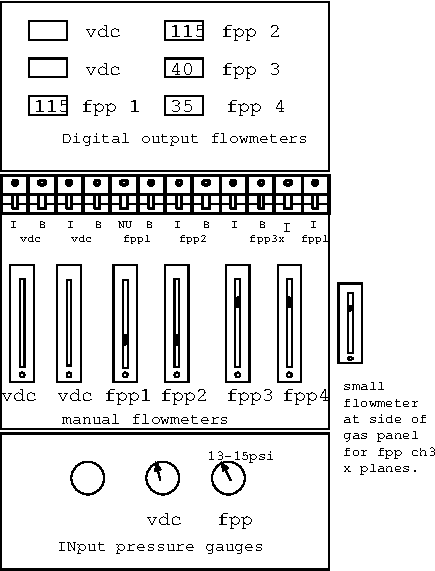
\includegraphics[angle=0,height=20cm,clip]{fpp_gaspanel}
{\linespread{1.}
\caption[Detectors: Hadron Arm Gas Panel]{Drawing of the gas panel on the hadron detector stack.}
\label{fig:gaspanel}}
\end{center}
\end{figure}


(The FPP chambers are also in parallel with the VDC chambers.)
All gas connections
are made using POLYFLO$^{TM}$ tubing and TJNAF-specified connectors.
The chamber volumes range from approximately
120 to 220 $\ell$.
Gas pressure in the chambers is typically a few Torr above atmospheric
pressure.
The gas flow through the chambers may be independently varied and is
typically set to 7 $\ell$/hr, leading to a replacement of the chamber
volumes about every 15 - 30 hours.
Gas is exhausted from the FPP chambers through a bubbler containing $<$ 1 mm
of mineral oil. A typical chamber leakage rate at this flow rate is 25 - 50
$\%$.
The flow rate of 7 $\ell$/hr when combined with the leak rate of
$\le$ 3 $\ell$/hr results in a complete exchange of gas in the chambers
roughly every 1 - 2 days.
At this level of consumption, a full gas bottle connected to the FPP system
lasts approximately 10 days.
When a bottle is nearing empty ($\approx$ 90$\%$), it should be changed since
there may be heavy contaminants in the gas.
Gas bottles may only be changed by authorized personnel.

\begin{center}
{\bf Gas-handling Procedures}
\end{center}

\begin{enumerate}
\item Typically gas is continually flowing though the chambers.
If at all possible, gas flow should be continuously
maintained, even in no-beam time periods.   This avoids time loss to
reconditioning and maintains the desirable steady-state operating
condition. If the chambers are not being used in an experiment, 
the flowmeters for the front chambers
are set to 20 and the flowmeters for the rear chambers are set to 60.
When the chambers are used in an experiment the standard setting
for the front chambers is 40 and for the rear chambers it is 105. 
\item Gas pressure at the gas panel on the 
detector stack should be in the range
13 - 15 psi. With the large leakage rate of the
FPP chambers, we typically run at near the limit of the capacity of the
gas mixer to supply the gas flow demanded by the FPP and VDC chambers.
Therefore it is possible to demand too much flow rate from the mixer.
If the gas pressure drops below 13 psi drop the flow to the FPP chambers
and contact Jack Segal or Howard Fenker to determine the cause and
remedy for the situation.
\end{enumerate}

The status of the gas handling system should be monitored carefully
as well as logged at least once per 8-hour shift.  Any substantial
deviation from the median parameters indicates a change in the
operational parameters of the FPP and should be immediately
investigated.  

\paragraph{Power Supplies and Electronics Procedures}

The power supplies and readout electronics associated with the FPP
are a mixture of commercially purchased equipment
and equipment designed and/or assembled with the Rutgers
University Department of Physics \& Astronomy Electronics Shop.
The reader is directed towards the manuals made available by the
manufacturer for the detailed information not provided here
for the commercial equipment.
For the Rutgers constructed equipment,
further documentation is available on the web page%
\htmladdnormallinkfoot{}{\url{
http://www.jlab.org/~gilman/fpp-homepage.html
}}.

\noindent
and through FPP notebooks (try for example contacting R.\ Gilman 
for notebooks maintained by Rutgers, CEBAF Center, phone 757.269.7011).

The LeCroy 1458 HV control crate houses the Lecroy  1469P modules
which control the HV for the FPP chambers. The 1469P has 3 master HV
channels and each master HV channel controls eight slave channels.
In slot 7 of the 1458 is the 1469P module 
which controls chamber~1 and chamber~2.
In slot~8 of the 1458 is the 1469P module 
which controls chamber~3 and chamber~4.
The individual slave channels can trip from high current faults
or other trip faults, but all eight slave channels must be raised and lowered
together by setting the master high voltage.
The HV provides +1.8 - 1.9 kV nominal to
each of the $\approx$ 5100 wires in the four FPP straw chambers.
The power supply is located in the detector stack at the top of
crate 6 in the upper electronics level.
This unit is controlled through HAC13.
Connections from the power supply to the chambers are made using
standard SHV connectors mounted on red RG-59/U HV cable good to 5 kV.

The high-current low-voltage supply boxes were assembled by Rutgers
University.
They are designed to provide a maximum current of about 1.6 / 0.6 A
at -5 / +5 V to each of the 318 readout cards on the four chambers.
There are 63 / 63 / 90 / 102 cards on chambers 1 / 2 / 3 / 4.
Typical operating currents are about two-thirds of this nominal
maximum value.
The +/-5 V power lines are independently fused to each card.
Each of the eight supply boxes contains two or three power supplies,
each rated for either 35 or 50 A.
There are two power boxes for each chamber.
Six boxes are located at the lower rear end of the detector stack.
The second boxes for chambers 3 and 4 are located at the top of the
detector stack, on an aluminum plate just off the upper electronics level.
These power boxes are monitored through EPICS, but turned on/off
though front panel switches.

Hewlett-Packard 6111A power supplies are used to provide typically
2 - 3 mA current per readout card.
Each of the front and rear chambers have their own power supply.  
The front chambers thresholds are fused, 
to limit current drawn in case of a short on the board.
The rear chamber cards use a 1.5 k$\Omega$ resistor external to the board
to limit current drawn, in case of a short on the board.
Board threshold circuitry also has a 1.5 k$\Omega$ to ground which
with the external 1.5 k$\Omega$ makes a voltage divider. Therefore,
the rear threshold supplies are typically set to a voltage which is
a factor of two larger than the front threshold supplies to give the
same threshold voltage at the readout board.
Initial tests indicate that at least a 1.5 V threshold must be applied to the
cards to prevent oscillations - this level will stop oscillations that arise
when the voltage applied is reduced to about 1.0 V.
In practice it has been found that the front chambers should be operated
at 4~V and the rear at 7~V. Efficiency studies show that the chamber
threshold could be raised by 50\% with minor loss in efficiency.
The HP supplies are also mounted in the hadron arm detector stack, on an
aluminum panel located beneath the two upper high current supplies.

Each straw wire contains a 25$\mu$m $\phi$, Au-plated
tungsten-rhenium wire.
The number of wires per plane varies from 176 to 272.
Wires are multiplexed 8 wires into one electronics channel,
leading to a required 636 TDC channels.
In practice a few extra channels are used, so that each 34 wire
(16 differential signal channels plus one ground pair)
twisted pair cable contains only signals from one of the four chambers.
LeCroy 1877 multihit FASTBUS TDCs are used to measure the leading edge time
and width of the pulses, to demultiplex the wire hit.
Within each group of eight wires, the widths are set to about
25, 45, 35, 55, 90, 65, 105, and 75 ns.
The TDCs are located in the upper FASTBUS crate located on the lower
electronics level of the spectrometer space frame in the detector hut.
The FPP rack, containing level shifter cards, is located opposite the
FASTBUS crates on the lower electronics level.
It shifts signals sizes from the reduced $\pm$50 mV readout card output levels
to ECL standard levels, for input to the TDCs.
The connections between the readout cards and the level shifter cards,
as well as between the level shifter cards and the TDCs,
are made with 16-conductor twisted-pair cables. 
A wiremap, detailing the cabling, is posted on the side of the FPP rack.

\begin{center}
{\bf Power-up Procedure}
\end{center}

\begin{enumerate}
\item {Ensure that gas flow has been established in the chambers as
outlined in the previous section.  If it has not, {\it STOP RIGHT
HERE!}  Gas flow must be well-established and steady-state
{\it BEFORE} the HV may be enabled.}
\item {Ensure that all power supplies as well as the FASTBUS crate
are off and the LV, HV, and TDC cables are connected.}
\item {Turn on the threshold and LV power supplies. Use EPICS to turn the
threshold voltages up to correct values, about 4.0 V for front chambers 
1 and 2, and 7~V for rear chambers 3 and 4.}
\item {Use HAC13 to turn up the chamber voltages. Standard
values are 1875 V for front and rear chambers.
It is probably best to raise the HV in 300V steps. After each
step wait for the current to settle below 1 $\mu$A, then
go up to the next level until 1875V is reached.
Peak currents during  turn-on should not exceed about 40 $\mu$A. 
A 10 V/s ramp rate leads to a leakage current of several $\mu$A.
Trip levels should be set to 110 $\mu$A both for turning on HV and
for normal operation, so that bad spills do not trip the chambers.
Current should settle to about a $\mu$A or less within a few minutes.
If the power supply trips during the ramping procedure, it
is possible that you are moving too fast, or that some
problem has developed with a chamber.
Rezero things and begin the procedure again.
{\it NEVER USE THE AUTO-RESET FUNCTION.}}  If
the power supply trips again, {\it STOP IMMEDIATELY AND INVESTIGATE.
There is probably a problem and expert advice may be needed.
Some detailed information, intended for experts debugging hardware
problems, is available in the Rutgers web pages. }
\item {Check for poor signal connections evidenced by hot wires (wires
counting extremely fast) or dead wires (wires with no counts) using
the histogramming software and cosmic rays.
Be careful: apparent problems may result from bad demultiplexing rather than
from poor signal connections.
Remake any connections as necessary by first powering down the FASTBUS crate.}
\end{enumerate}

If at all possible, the HV and LV power supplies should be left
on continuously if and only if gas is available to the chamber.  This
avoids time loss to reconditioning and maintains the desirable
steady-state operating condition.


\section{Carbon Doors}


Four of the five doors operate remotely, the fifth needing further
testing before it is certified reliable. The
doors use the EPICS control system to activate and read back the
various components. 

Each layer of carbon doors has one relay board. 
Each board is identical in operation and
there is one spare in the event one of them should fail. The global
purpose of the relay board is as follows:

\begin{enumerate}
\item Turn on the 12V to power to rest of circuit board.

\item Set the polarity on the 90V used to power the motors.

\item Turn the 90V on.

\item Cut off the 90V to a motor if the appropriate limit switch is
hit.

\item Read back the status of the limit switches.
\end{enumerate}

The 12V used to power the circuit board runs through this relay and it is
activated via an EPICS relay in VME crate 4 (hallasc4). Relay \#1 turns
on the 90V and it too is activated by an EPICS  relay in VME crate 4.
Relay \#2 switches the polarity of the 90V being fed to the driving
motors. When activated it reverses the polarity to the motors and it is
controlled by a relay in VME crate 4. Relays \#3 and \#5 are activated by
the inner limit switches of the carbon doors. When these switches are
depressed the relay activates and the 90V is cut off. Relays \#4 and \#6
are activated by the outer limit switches of the carbon doors and like
relays \#3 and \#5 cut off the 90V when activated. Relays \#4 and
\#6 activate when opened rather than when depressed.
It would be nice in the
future to have relays \#3 and \#5 also activated by an open limit
switch condition and deactivated when the switch is closed. This way
the 12V could be off to one of the switches and the doors would stop
moving. As it is now, a broken wire/short while the doors are
closing could cause the doors to continue moving risking possible damage.


The status of the limit switches is readout via an ADC in VME crate
4. If the switches are closed a -4V is seen at the ADC input. This is
effected via a voltage splitter of 3 k$\Omega$ - 6 k$\Omega$ resistors. The
readouts are plugged in via telephone jacks (PJ4, PJ5, PJ6, and PJ7). A
temporary fix has been put in place which sends the signals through a
capacitor first to block voltage spikes going into the ADC. These
voltage spikes caused the ADC to trip off-line which can only be
fixed by resetting the VME crate.

\begin{figure}
\begin{center}
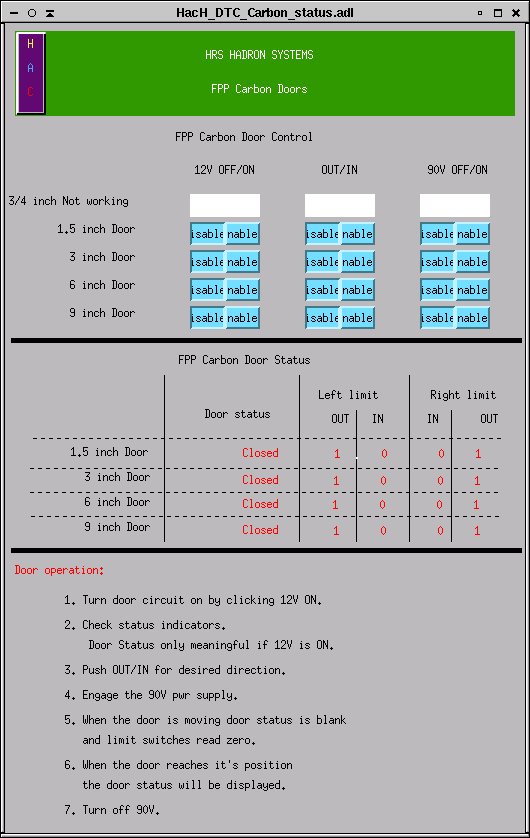
\includegraphics[angle=0,height=21cm,clip]{medm_halla_fpp_doors}
{\linespread{1.}
\caption[Detectors: FPP Carbon Door GUI]{EPICS GUI for the carbon doors.}
\label{fig:carbon_door_gui}}
\end{center}
\end{figure}

The operation of the carbon doors is done via a GUI style control
panel . This panel is located under the detector screen of the hadron
arm (FPP Carbon Doors). The 3/4" carbon door has been disconnected at
the 90V power supply and is not implemented in the software GUI. This
door had what may have been some sliding problems. Since it may take a
great deal of force to remove this door if it should jam, it will need
to be tested so it can be removed easily if it should jam. The normal
operating procedure with the GUI is to first
make sure all the 90V
power is off to each door (Blue switches), then to
turn on the 12V power to each door to see where it
is located in the stack (in vs.
out). If you wish to change the status of a door (in/out) then simply
toggle the IN/OUT switch appropriately and  turn on the 90V. It takes
some time for the doors to move the entire range, so be patient. When
the limit switches have been reached the appropriate indicators will
light up. You should then turn the 90V off. The important aspect of
this procedure is to make sure that you do not change the polarity of
the 90V while the doors are moving. This place undue stress on the
motors and the power supply as well.

\section{Handling Considerations}

The FPP straw chambers are very delicate devices which are absolutely
essential to many Hall A physics experiments.
Thus, extreme care must be taken whenever they are moved or used.
Also, extreme care must be taken that other objects are not moved
into them.

\begin{itemize}

\item{Before moving a straw chamber, ensure that any protective
plates are in position.}

\item{Disconnect and reconnect all TDC, HV, and LV cables with care.}

\item{When initiating gas flow, pay strict attention to the feedback
parameters.
Straw chambers are not very sensitive to overpressure of perhaps
50 - 100 Torr,
but {\bf the straw chambers can be easily destroyed by a few Torr 
underpressure}. }

\item{Never attempt to apply HV to the chambers until gas flow
conditions have reached steady-state.}

\item{As the amount of heat generated by the pre-amp/discriminator
cards is substantial, always make sure adequate cooling is provided
before attempting to run.
This is mostly ensured by making certain that the various
cooling holes through the Faraday shields are not covered.
The chambers have internally mounted fans where needed, which
are powered up along with the readout cards.}

\item{If the leakage current on the high voltage rises linearly
with voltage, then a wire has broken and
is shorted to ground!}

\end{itemize}

} %infolev

\begin{safetyen}{0}{0}
\section{Safety Assessment}
\label{sec:fpp_safety}
\end{safetyen}

\begin{safetyen}{10}{10}
The following potential hazards have been clearly identified.

\begin{description}

\item {\bf The High Voltage System}
The LeCroy 1458 HV low current power supply provides a nominal
+1.80 kV.
Red HV RG-59/U cable good to 5 kV with standard SHV connectors is used
to connect the power supply to the chambers.
Each HV channel, of the 6 per chamber, typically will draw a few hundred nA.

\item {\bf The Low Voltage System}
LV power supplies are used for the pre-amp/discriminator/multiplexer
cards.
Each card requires up to 
1.6 A at -5 V and 0.6 A at +5 V, plus a few mA threshold at 4 - 8 V.

\item{\bf High Pressure Gas Bottles} The  gas used 
in the chambers is supplied in high pressure ($\ge$ 2000 psi) gas
bottles. This confined high pressure gas represents a tremendous
(potentially lethal) amount of stored energy.
\end{description}
\end{safetyen}

\begin{safetyen}{10}{15}
\section{Authorized Personnel}
\end{safetyen}

The individuals shown in Table \ref{tab:fpp:personnel} are responsible for 
chamber problems. Generally, the non Jefferson Lab people are responsible for
FPP detector problems, whereas the Jefferson Lab people are responsible
for more general data acquisition problems or, e.g., gas / voltage supplies
shared with other systems.
\begin{namestab}{tab:fpp:personnel}{FPP: authorized personnel}{%
      FPP: authorized personnel.}
  \BogdanWojtsekhowski{\em Contact}
  \SirishNanda{}
%  \RonaldGilman{}
%  \CharlesPerdrisat{}
%  \VinaPunjabi{}
%  \XiaodongJiang{}
  \JackSegal{}
\end{namestab}

%\vfill\eject
